\documentclass[tikz]{standalone}
\usepackage{tikz}
\usetikzlibrary{positioning, graphs}
\usetikzlibrary{graphs.standard}
\begin{document}
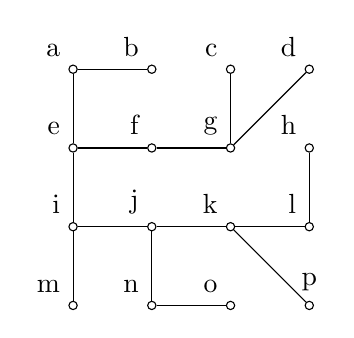
\begin{tikzpicture}
\begin{scope}
		[vertex/.style={draw,circle,inner sep = 0em, minimum size = 0.3em},
		 edgelabel/.style = {fill = white, inner sep = 0.1em, font=\small}]
		\node[vertex, label = above left : a] (a) at (0,0) {};
		\node[vertex, label = above left : b] (b) at (1,0) {};
		\node[vertex, label = above left : c] (c) at (2,0) {};
		\node[vertex, label = above left : d] (d) at (3,0) {};
		\node[vertex, label = above left : e] (e) at (0,-1) {};
		\node[vertex, label = above left : f] (f) at (1,-1) {};
		\node[vertex, label = above left : g] (g) at (2,-1) {};
		\node[vertex, label = above left : h] (h) at (3,-1) {};
		\node[vertex, label = above left : i] (i) at (0,-2) {};
		\node[vertex, label = above left : j] (j) at (1,-2) {};
		\node[vertex, label = above left : k] (k) at (2,-2) {};
		\node[vertex, label = above left : l] (l) at (3,-2) {};
		\node[vertex, label = above left : m] (m) at (0,-3) {};
		\node[vertex, label = above left : n] (n) at (1,-3) {};
		\node[vertex, label = above left : o] (o) at (2,-3) {};
		\node[vertex, label = above : p] (p) at (3,-3) {};
		
		\draw[-] (a) to (b);
		\draw[-] (a) to (e);
		\draw[-] (c) to (g);
		\draw[-] (d) to (g);
		\draw[-] (e) to (f);
		\draw[-] (e) to (i);
		\draw[-] (f) to (g);
		\draw[-] (h) to (l);
		\draw[-] (i) to (j);
		\draw[-] (i) to (m);
		\draw[-] (j) to (k);
		\draw[-] (j) to (n);
		\draw[-] (k) to (l);
		\draw[-] (k) to (p);
		\draw[-] (n) to (o);
\end{scope}
\end{tikzpicture}
\end{document}